\chapter{Leveraging Social Context for Topic Evolution}
\label{kdd_chapter}
Topic discovery and evolution (TDE) has been a problem which has gained
long standing interest in the research community.  The goal in
topic discovery is to identify groups of keywords from large corpora so that the information in those
corpora are summarized succinctly.  The nature of text corpora has changed
dramatically in the past few years with the advent of social media.  
Social media services allow users to constantly share, follow and comment
on posts from other users.  Hence, such services have given a new
dimension to the traditional text corpus.  The new dimension being that
today's corpora have a \emph{social context} embedded in them in terms of the
community of users interested in a particular post, their profiles etc.  
We wish to harness this social context that comes along with
the textual content for TDE.  In particular, our goal is to both
qualitatively and quantitatively analyze when
social context actually helps with TDE.
Methodologically, we approach the problem of TDE by a proposing non-negative matrix
factorization (NMF) based model 
that incorporates both the textual information
and social context information.  We
perform experiments on large scale real world
dataset of news articles, and use Twitter as the platform providing information
about the social context of these news articles.
We compare with and outperform
several state-of-the-art baselines. Our conclusion is that using
the social context information is most useful when
faced with topics that are particularly difficult to detect.
\section{Introduction}
\label{sec:introduction}
\section{introduction}
Social media has changed our way or looking at information. From simple consumers we have been given the opportunity to produce and act on what is potentially trending now. Each of us can  inform, comment,m and participate in his own way to the constant flow of events that apparently never ends. 

As a matter of fact, the overload of information caused by the always growing flow of stories have been subject of an uncountable number of studies \cite{}. Among which some have tried to leverage and select information adapted to the final end user \cite{}. This is particularly the case for the online media industry who have been facing many new challenges with the shift from the printed to online press. One challenge of interest is the ability to discover and track along time news events. For instance, both media internet actors, Yahoo and Twitter, propose  on their homepage a \emph{``trending now"} module aiming at helping the user to focus on the most dominant topic in the big flow of information.

Topic detection and tracking (TDT) is a subject of large attention since more than a decade \cite{} but have gained recently new interest with the advent of the social media.  TDT aims at detecting along time the main trends in flow of information and at giving to each of them a short description. By doing so, media actors can help the end user in following how topics emerge, evolve and fade. By connecting topics along time the end user is provided with a map helping him to deal with information overload.

The most effective models developed by the TDT community consists of an extension of  topic models where the time information is taken into account. This is the case with  recently introduced  NMF based models --- used traditionally for topic modeling --- by connecting along time the learned representations as the flow of document is produced \cite{}. In the same spirit, other works extend LDA for analyzing the evolution of topics along time \cite{}. However, these last approaches by relying on full bayesian modeling are  too slow to be used in practice \cite{}.


All TDT approaches  still consider to observe as input  only a flow of raw textual information. Actually, there are blind to the fact that  nowadays  information on the social media comes with metadata giving it a social context. In this work, we argue that by leveraging this social information along with the content one can track topic evolution along time in a more accurate way. For instance, it make sense to believe that when  \emph{lionel messi or christiano ronaldo} is mentioned in a tweet it is more likely that this is a tweet about football than politic. While when \emph{Obama} tweets about \emph{employment growth} it is more likely to be about politic. 

To the best of our knowledge, while using social metadata has been considered for the task of topic modeling \cite{}, it has never been considered for tracking topics along time. Therefore, we propose a novel topic tracking model to be used in a streaming environement to discover and track topic along time. Our model relies on the idea of collective matrix factorization (CMF)  by learning shared representations from both the tweet content information and from the social media information coming along with the tweet (i.e. the author and the mentions). By doing so, we learn in the same time the topics but also the communities (i.e. group of users) supporting each of the discovered topic. Our model, inspired from \cite{},  gives the possibility to connect topics and communities along time. The model is designed such that we  can set a joint or a distinct evolution pattern for topics and communities. We show that depending on the nature of the topic some exhibits a common evolution pattern with their supporting communities,  while others exhibits unrelated patterns.   We test to which extent  by using the social media context of the tweet discover better topics. We show that this is particularly the case  for \#tags that exhibit a big variation in their topics while being stable in terms of community (i.e. users engaged with this #tag).







\section{Comparison to previous work}
\label{sec:comparison_to_previous_work}
\input{KDD/comparison_to_previous_work.tex}

\section{Learning from content and social media activity}
\label{sec:content_and_networks}
\input{KDD/content_and_networks.tex}

\section{DATA SET DESCRIPTION}
\label{sec:data_set_description}
\input{KDD/data_set_description.tex}

\section{Experiments}
\label{sec:experiments}
\section{Timeline Generation: The Methodology}
\label{sec:timeline_generation}
\begin{figure*}
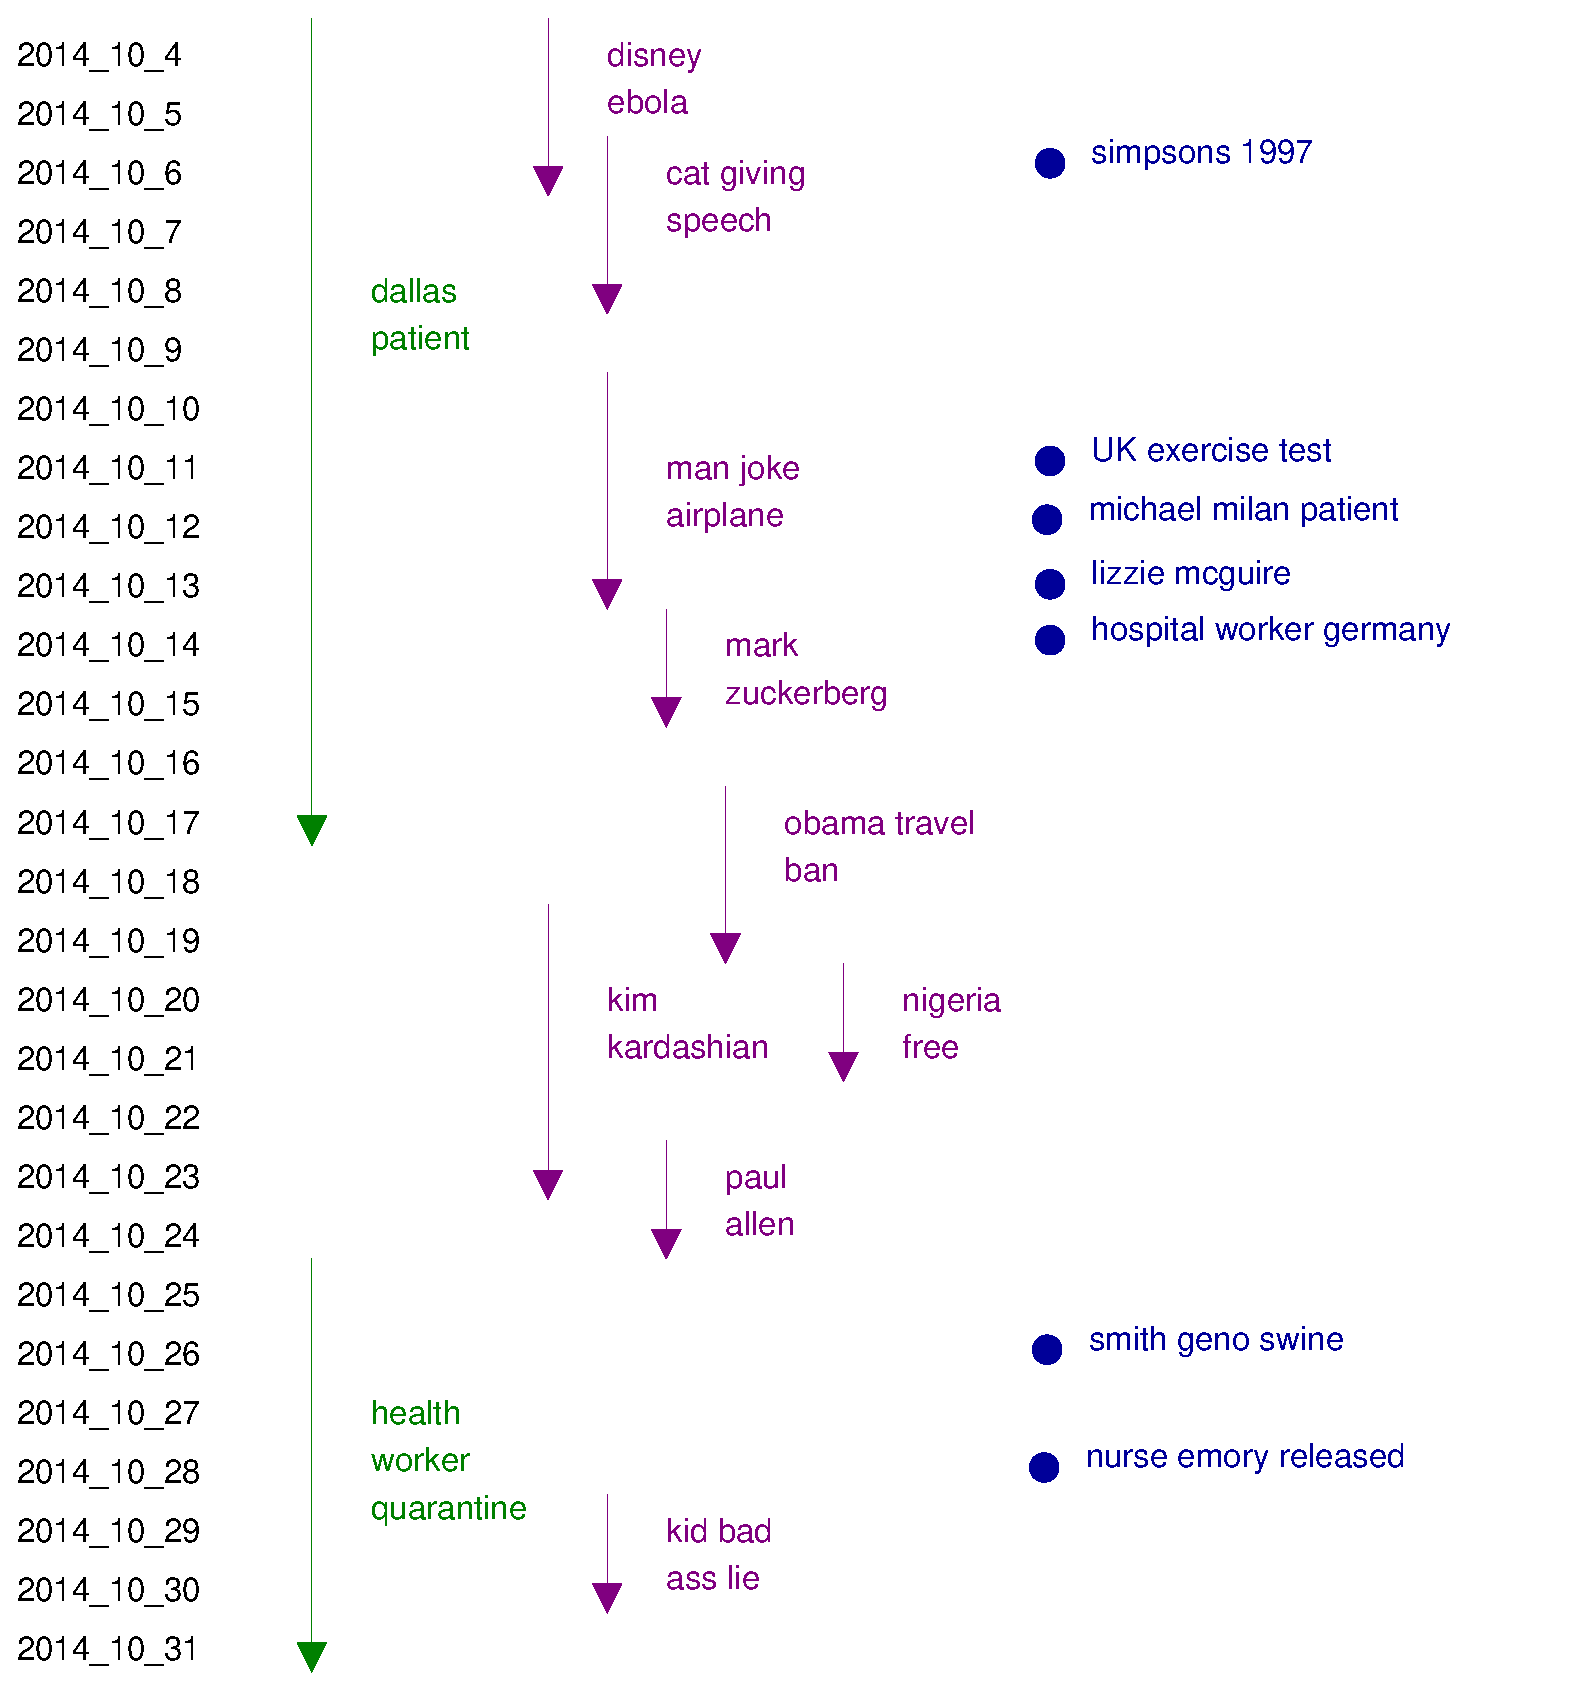
\includegraphics[width=\textwidth]{ICWSM/figures/timeline.eps}
\caption[Ebola: Timeline of events]{Ebola Timeline of Events on Twitter}
\label{fig:timeline}
\end{figure*}
The following steps were taken to generate a timeline of events:
\begin{enumerate}
\item the data was chronologically sorted and split into smaller blocks covering 24 hour timesteps (Section \ref{subsec:data_split});
\item topic modeling approaches were applied on each block, to obtain a set of topics (Section \ref{subsec:topic_models});
\item the set of topics identified in each block was mapped to the topics of the previous block. Such a mapping of topics over time is
referred to as an \emph{event}.  If a topic did not match any topic in the previous block, it was marked the beginning of a new event (Section \ref{subsec:topic_maps}).
\end{enumerate}
To generate the final timeline for event category and longevity analysis, 
we combined the results from steps (2) and (3) above.
We used two different topic modeling algorithms, \cite{Yan:2013:BTM}'s \emph{Biterm Topic Model} (BTM), and a novel variant
of non-negative matrix factorization which we propose in this work to explicitly model and identify
new, fading and changing topics.  To gain further insights into the characteristics and quality of topics output by each algorithm, we performed a quantitative evaluation (see Section 5).  

\subsection{Splitting the Data}
\label{subsec:data_split}
In order to track topics over time,
we split the tweets into smaller blocks pertaining to a particular time period, and apply
topic modeling on each smaller block to obtain the important topics during that time period.
In order to decide on the resolution of the smaller blocks of tweets, we look at volumes
of tweets versus time, see Figure \ref{fig:vol_time}.
The \texttt{x-ticks} coincide with approximately 5AM Eastern Standard Time.
We observed that,
starting at about 5AM Eastern Standard Timei every day, there is a gradual increase in the volume of tweets
with peak volume from around 3PM to 6PM Pacific Standard Time, with volume gradually decreasing
after 6 PM.  This pattern is
stable across all the days in our dataset, and also consistent with the general tweeting behavior
as reported in other studies such as \cite{liu:2010, java:2007}.  This tells us that come what may,
the rate of tweet production decreases at night, and gradually increases as the day breaks.
Hence, we split the data into one-day periods corresponding to the Eastern Time Zone of the United States.


\subsection{Topic Models}
\label{subsec:topic_models}
Note that our corpus has some distinct characteristics.  One, it is a corpus with
documents which are extremely short in length (about 5 words per tweet).  Two, there is
a temporal aspect to the corpus since the data is split into time intervals of $1$-day.
It is hence important for the topic model to be able to learn from extremely short texts.
Furthermore, it may be useful for the topic model to exploit any knowledge gained from the previous timestep.  

Any conventional topic modeling algorithm like latent dirichlet allocation and its
derivatives \cite{blei2003}
or probabilistic latent semantic analysis \cite{deerwester1990indexing} do not work well on corpus
of short text \cite{Hong:2010, Jin:2011, Zhang:2013}.  The main reason is that such topic models capture word co-occurrences at the document
level.  When the documents are very short, these topic models suffer from sparsity issues.

We use two topic modeling algorithms to discover the topics.  We propose the first
topic model, called \emph{t-short} (stands for \emph{temporal-short-text}) which is specifically geared toward short texts,
and explicitly models the evolution of topics over time by categorically identifying
them as new, fading, or evolving.  On a high level, \emph{t-short} is based non-negative matrix factorization
with 
a temporal concept added to it.  The second topic model which is based on
latent dirichlet allocation, but modified for short texts, is called Biterm Topic
Model (\emph{BTM}) and is proposed by \cite{Yan:2013:BTM}. 
These two models are further described below.

\subsubsection{T-Short}
A non-negative matrix factorization performed on a term-document matrix $\textbf{X}$ is a conventional
approach to obtain the underlying latent topics in the corpus.  However, when the length of the documents
is very short as in our case, this matrix $\textbf{X}$ suffers from sparsity.  

One observation to be made about corpora of short texts is that the rate at which the
size of the vocabulary grows is generally much slower than the corresponding
number of documents.
In some sense, a very large number of documents are being generated from a relatively
small vocabulary.  This results in
the word co-occurrence matrix $\textbf{K}$ (a square matrix, with dimension equal to the size of the
vocabulary, which models some notion of normalized co-occurrences) 
being comparatively denser than the term-document $\textbf{X}$.  
Factorizing this matrix would result in:
\begin{eqnarray}
    \textbf{K} \approx \textbf{Q}^{T}\textbf{Q}. \label{eq:learning}
\end{eqnarray}
Equation \ref{eq:learning} can be thought of as a clustering of commonly co-occurring words 
into coherent topics.  
In our paper, we consider the squared loss $||\textbf{K} - \textbf{Q}^T\textbf{Q}||_F^2$
and factorize the $m$-by-$m$ word co-occurrence matrix $\textbf{K}$ symmetrically into 
an $m$-by-$k$ topic matrix $\textbf{Q}$, where $k$ is the number of topics.  Like in any topic model, the parameter $k$ of the number of topics
needs to be set manually (generally by cross-validation).
This is called symmetric 
non-negative matrix factorization \cite{Kuang:2012}.
Such a factorization has shown to improve performance in terms of topic discovery
over the conventional factorization of the $\textbf{X}$ matrix \cite{Yan:2013}.

Since we are faced with a stream of data in $1$-day time intervals, we consider a series of
matrices $\{\textbf{K}^t\}_{t=1}^{t=T}$.  While factoring $\textbf{K}^t$, we would like to 
exploit the knowledge gained in time-$(t-1)$.  We do so by considering the following
formulation of matrix factorization:
\begin{eqnarray}
L = ||\textbf{K}^{t} - {\textbf{Q}^{t}}^{T}\textbf{Q}^{t} ||^2_F+ ||\textbf{K}^{t} - {\textbf{Q}^{t}}^{T}\textbf{M}^{t}\textbf{Q}^{t-1}||^2_F + \alpha(R). \label{eq:evolution}
\end{eqnarray}
In Equation \ref{eq:evolution}, the quantities $\textbf{K}^t$ and $\textbf{Q}^{t-1}$ are considered known.  The unknowns are
$\textbf{Q}^t$ and $\textbf{M}^t$\footnote{$R$ stands for regularization of all the variable quantities.  
We apply the $l$-1 norm regularization on
$\textbf{Q}^t$ and $\textbf{M}^t$.}.  Here, the first term is similar to the squared loss from Equation \ref{eq:learning}.
The second term factors the $\textbf{K}^t$ matrix given the knowledge of the topics from time-$(t-1)$ (through
the $\textbf{Q}^{t-1}$).  Here, the $\textbf{M}^{t}$ matrix can be viewed as enabling a \emph{smooth} transition
from one time step to another.  

To see the purpose of the $\textbf{M}^t$ matrix more clearly, we can think of $\textbf{Q}^t \approx \textbf{M}^t\textbf{Q}^{t-1}$.
Note that $\textbf{M}^t$ is a $k$-by-$k$ matrix.  Note also that the entries of $\textbf{M}^t$ are all positive.  
Hence, the $i$-th row of $\textbf{M}^{t}$ helps explain the $i$-th topic for time-$t$ as a mixture of the previous topics.
If a particular row of $\textbf{M}^t$ is $\textbf{0}$, it means that particular topic is new (since it cannot be
explained by any of the previous topics).  If a particular column of $\textbf{M}^t$ is $\textbf{0}$, it means that this
particular topic is fading topic since it has not found its presence anywhere at time-$t$.  
The idea of using transition matrices to \emph{track} quantities have been used before \cite{Kalyanam:2015,Vaca:2014}.
However, to our knowledge, this is the first time it is being proposed in the context of modeling topics over short text.  

We optimized Equation \ref{eq:evolution} using multiplicative updates.
To optimize the loss in Equation \ref{eq:evolution}, we considered the two identical factors in the first term 
to be different.  Assuming that one of the $\textbf{Q}^t$ matrices was known, we updated the other.  
We then update the $\textbf{M}^t$ matrix with the newly updated $\textbf{Q}^t$ matrix.  

\subsubsection{Biterm Topic Model}
The Biterm Topic Model (or BTM) model was proposed by \cite{Yan:2013:BTM} to uncover topics from corpora
of short texts (like instant messages and tweets).  It is similar to latent dirichlet
allocation \cite{blei2003} in its graphical model.  The main difference is that it
models the generation of \emph{biterms} instead of just the singular terms.  The motivation
for modeling the occurrences of biterms is to address the sparsity issue which latent dirichlet
allocation suffers from when applied to corpora of short texts.

\subsection{Mapping the Topics}
\label{subsec:topic_maps}
\begin{figure}
\includegraphics[width=0.4\textwidth]{ICWSM/figures/heatmap_t_7_8.eps}
\caption[Heatmap of transitions]{A colored heatmap of the matrix $\textbf{M}^t$, where $t = 5$.
The top words from each of these topics are shown in Table \ref{tab:topics_7_8}.}
\label{fig:heatmap_7_8}
\end{figure}
\begin{table}[h]
\tiny
\centering
\begin{tabular}{c c}
\hline
\pbox{20cm}{topic\\ at $(t-1)$} & \pbox{20cm}{top words}\\
\hline
1& patient, people, virus, dont, health \\
2& africa, patient, people, first, virus, dont\\
3& spain, nurse, virus, africa\\
4& dont, cat, patient, giving, speech\\
5& spain, spanish, nurse, africa\\
\hline
\pbox{20cm}{topic\\ at $(t)$} & \pbox{20cm}{top words}\\
\hline
1& cat, giving, speech, presidential\\
2& first, patient, died, thomas, eric, duncan, breaking\\
3& hospital, patient, admitted, carlos, infections\\
4& africa, patients, outbreak, airports, world, travel\\
5& spanish, nurse, infected, face, touched\\
\hline
\end{tabular}
\caption[Top words to illustrate topic transitions]{This table presents the top few words from each of the $5$ topics
obtained from \emph{t-short} at the dates $2014/10/7$ (represented as topic-$t$) and $2014/10/8$ (represented
as topic-$(t+1)$.  This table must be studied in conjunction with Figure \ref{fig:heatmap_7_8}.}.
\label{tab:topics_7_8}
\end{table}
\begin{table}[h]
\tiny
\begin{tabular}{|c|c|c|c|c|c|}
\hline
\multicolumn{6}{c}{time-$t$} \\
\hline
Topic ID& topic-1 & topic-2 & topic-3 & topic-4 & topic-5 \\
\hline
&people & cdc& disney& patient &africa\\
&dont & possible& ur& hospital&akon\\
&amp & newark& watching & dallas&bubble\\
&virus & passenger& channel & critical&disease \\
&obama & airport & watchin & texas&virus\\
&seconds & symptoms &  chanel & condition & hits \\
&retweet & official & merica & bae & tweets \\
&stop & flight & shit & case & fight \\
&america & plane & season & family & blunt \\
&gonna & breaking & football & home & kill \\
\hline
\hline
\multicolumn{6}{c}{time-$(t+1)$} \\
\hline
\pbox{20cm}{Topic ID \\from time-$t$}&\pbox{20cm}{topic-3 \\from \\time-$t$} & \pbox{20cm}{topic-5 \\from\\ time-$t$} & \pbox{20cm}{new topic} & \pbox{20cm}{topic-1 \\from\\ time-$t$} & \pbox{20cm}{topic-4 \\from\\ time-$t$} \\
\hline
&ur & hits & hospital & people & patient \\
&watching & kill & patient & dont & dallas \\
&disney & blunt & tonight & virus & cdc \\
&channel & germs & oct & amp & man \\ 
&disease & africa & simpsons & shit & case \\ 
&seconds & fight & 1997 &  jokes & health \\ 
&tweets & outbreak &  19 &  back & officials \\ 
&quicker & america & predicting &africa & homeless \\
&spreadin & united & goodluck & yall & outbreak \\
&retweets & hand & sleeping & u & first \\
\hline
\end{tabular}
\caption[Manual topic-by-timestep mapping example]{Manual topic-by-timestep mapping example, based on topics generated from the \emph{BTM} model.
The number of topics was set to 5.  The table represents a slice of the set of topics obtained on 
$2014/10/04$ (represented as time-$t$) and the set of topics obtained on $2014/10/05$ (represented
as time-$(t+1)$).}
\label{tab:BTM_mapping}
\end{table}
Once we have the topics for each block of tweets, the next step is to map the
topics across time to create a topical timeline, an event.
Our algorithm \emph{t-short} has the evolution matrix
$\textbf{M}^t$ at every time step which can be analyzed to determine which
are the continuing, new and fading topics.  As
explained in Section \ref{subsec:topic_models}, row-$i$ of the $\textbf{M}^t$ matrix
tells us how topic-$i$ at time-$t$ is composed of the previous topics.  Thus, by examining
this $\textbf{M}^t$, we will be able to map the topics from the previous timestep
to the current.  We provide an example of this in Figure \ref{fig:heatmap_7_8} and
Table \ref{tab:topics_7_8}.  Let us study Table \ref{tab:topics_7_8} first.
At time-$t$, topics $2$ and $3$ seem to be new topics since they do not appear
to have any similarities with any topic from time-$(t-1)$.  Correspondingly,
in Figure \ref{fig:heatmap_7_8}, note that row-$2$ and row-$3$ are completely
zeroed out -- thus indicating that these two topics are new.  Also, from Table \ref{tab:topics_7_8},
it is clear that topic $4$ at time-$t$ is almost the same as topic $2$ at time-$(t-1)$.  This
is also represented through the matrix in Figure \ref{fig:heatmap_7_8} since the second entry
in row-$4$ is very high.  Similarly, by comparing the figure and the table, one can
easily conclude that topic $5$ at time-$t$ is indeed a combination of topics $2$, $3$ and $5$
from time-$(t-1)$.  We used such examination of the $\textbf{M}$ matrix to map the topics
from one timestep to another, and produced timelines for topics.

The \emph{BTM} algorithm, on the other hand, does not have any temporal aspect to it that automatically
maps topics from one timestep to another.  
To produce a timestep topic mapping from this model, 
a manual coding strategy was employed. 
Two of the coders mapped each topic of a
given time step to a topic of the previous 
time step. If a map was not found, it was marked 
as the beginning of a new
topic.
At each time step, they considered the top-$10$ words of each topic produced
by \emph{BTM}, and looked for a similar set of words in the previous timestep.
The agreement between the markings was $74\%$.  We give an example of their markings
in Table \ref{tab:BTM_mapping}.  Here, in time-$(t+1)$, there is a topic that is marked
as new.  On further investigation (through searching on Google, and Twitter), we found
that this topic was a meme which began on $2015/10/5$ about how an Ebola outbreak
was predicted in one of the episodes of the TV show \emph{The Simpsons}.  
Based on a qualitative examination of the mappings, it was clear that 
both coders were informally assessing the extent of 
lexical overlap between topics to determine topic trajectories.

\subsection{The Final Timeline}
Through the previous steps, two initial timelines of the Ebola as manifested on
Twitter were created.
A close examination of both timelines revealed that they were similar, but not identical.
There were some topics
that were not discovered by \emph{BTM}, but appeared in \emph{t-short} and vice versa.  
By using
a union of all the events in both the timelines, we produced
the final timeline presented in Figure \ref{fig:timeline}.
Each arrow
or a dot represents a single event.  The group of words listed next to the
arrow or dot were chosen from the top-10 words produced by the topic models
across the days that the event was active.  We chose those words that best
represented the event.
We call these words
the \emph{representative terms} of the event.

\section{Quantitative Evaluation of Topic Modeling Algorithms}
\label{sec:comparison}
\begin{table}
\centering
\begin{tabular}{|c|c|c|c|c|}
\hline
\#-topics & Score & \emph{t-short} & \emph{BTM} & \emph{LDA}\\
\hline
5 & NDCG & 0.2517 & 0.2209 & 0.1834\\
 &MAP &  0.1563   &  0.0944 & 0.0569\\
\hline
7 & NDCG & 0.2840 & 0.2327 & 0.1783 \\ 
 & MAP & 0.1789 &  0.1104 & 0.1093 \\
\hline
10 & NDCG & 0.2737 & 0.1974 & 0.1596\\
& MAP & 0.1801 & 0.0893 & 0.0345\\
\hline
\end{tabular}
\caption{This table shows the scores of the topics discovered by our algorithm \emph{t-short} on a groundtruth
obtained from considering hashtags to the scores of topics developed by other algorithms \emph{sym-NMF}
and \emph{BTM}.}
\label{table:groundtruth_table}
\end{table}
Before analyzing
the timeline, we will assess the performance of the
models; i.e., we try to evaluate the quality of results produced by
\emph{t-short} and \emph{BTM}.

It is generally a difficult task to evaluate the quality of topics
produced by a model \cite{chang2009reading}, leave alone the timeline.  
If there were some means
of obtaining the actual latent topics present in a time-sensitive corpus
like ours, one could compare
the results obtained by one's model to this groundtruth.  But such gold standard,
as in our case, is often not available.  

In this section, as a preliminary step to evaluating the performance of our
models, we choose to use \emph{hashtags} as a proxy for the groundtruth
topics. A \emph{hashtag} on Twitter is a sequence of characters followed by the `\#' symbol.  This
sequence of characters is generally associated to a meaningful word,
phrase or event and is conventionally used to give context to a tweet.
The user who posts
the tweets manually and optionally embeds a hashtag in the tweet.  In this study,
we exploit this usage of hashtags to serve as the groundtruth annotation
for the topic of the tweet.
Such an assumption has been proposed before (e.g. \cite{tsur2012s}) where
hashtags have been suggested to be used as groundtruths for evaluating topic models.
We extract the top hashtags at each timestep from 
our corpus to create a groundtruth, and evaluate the performance 
of \emph{t-short} and \emph{BTM} against this.

Note, however, that in order use hashtags as groundtruth annotations for topics,
we can only consider those tweets which indeed have a hashtag embedded in
them.  In our dataset (10.5M tweets in total), only 2.7M (25\%) have hashtags
embedded in them. This subset constitutes our groundtruth for this evaluation.

To obtain the groundtruth topic matrix, $\textbf{Q}_\text{groundtruth}$, 
the top-$m$ hashtags in each day were extracted, and used to obtain a bag-of-words 
representation of all the tweets which had any of
those $m$ hashtags embedded in them.
Each row in $\textbf{Q}_\text{groundtruth}$ matrix corresponds to the topic of
a particular hashtag.  This row was obtained by just taking the average of all the bag-of-words representations of the tweets
which had that particular hashtag embedded in them.  

It is a generally accepted norm that the top few words of a topic give good insight
about it \cite{newman2010automatic,sekiguchi2006topic}.
To evaluate how similar two topics are, we took the top-$10$ most likely words in each topic and
obtained two rankings.  
The rankings were evaluated by using two standard ranking measures: Normalized
Discounted Cumulative Gain and Mean Average Precision

As a baseline, we apply a regular \emph{LDA} model on the groundtruth subset, 
to compare with \emph{t-short} and \emph{BTM}. 
The results from this evaluation is presented in Table \ref{table:groundtruth_table}.
We observe 
\emph{t-short} and \emph{BTM} consistently outperform \emph{LDA}.
This corroborates that topic models developed specifically for short texts
indeed perform better than conventional models.  Also, note that
\emph{t-short} consistently performs better than \emph{BTM}
suggesting that \emph{t-short} is able to effectively capture those topics which are hashtagged by users.
This is also the only model
which incorporates the temporal information from the past
demonstrating the likely utility of using a model capable of leveraging temporal information.

\section{Timeline Analysis and Discussion:  Topics and Longevity Patterns}
\label{sec:timeline}
The timeline in Figure \ref{fig:timeline} was produced using the methodology
outlined in Section \ref{sec:timeline_generation}.  
In an effort to understand the characteristics of these
events, we divided them into three categories based on their longevity: the \emph{long-term} events (or) those
which lasted for $5$ or more days, \emph{medium-term} events (or) those which lasted
for $2$ to $4$ days, and \emph{short-term} events (or) those which lasted for $1$ day.

A few examples from each category were further examined to obtain a more 
comprehensive analysis, by extracting representative terms from the 
subset of tweets for the period under consideration along with the 
top two or three results from an Internet search using the 
Google search engine in the following way: 
\[
\texttt{representative terms} + \texttt{ebola} + \texttt{<date>}.
\]
These search results provided additional, external information about the context from which the timeline events originated.

\subsection{Long-term Events}
We found two \emph{long-term} events in our dataset.  One about \texttt{dallas patient}
and another about \texttt{health worker quarantine}.

\subsubsection{Dallas Patient}
\begin{table}
\begin{tabular}{c | c | c}
$2014/10/05$ & critical, condition, homeless, man, contact\\
$2014/10/06$ & nebraska, experimental, drug  \\
$2014/10/07$ & kidney, dialysis  \\
$2014/10/08$ & thomas, eric, duncan, died, first, patient \\
$2014/10/09$ & died, patient \\
$2014/10/10$ & duncan, fever, nurse \\
$2014/10/11$ & nurse, symptoms \\
$2014/10/12$ & health, care, worker, positive \\
$2014/10/13$ & health, care, worker, protocol \\
$2014/10/14$ & nurse, dallas, nina, pham \\
$2014/10/15$ & health, care, worker, 2nd, positive \\
$2014/10/16$ & nurse, flight, ohio \\
$2014/10/17$ & virus, flight, nina, pham \\
\end{tabular}
\caption{This table lists some of the top words that occurred in the event Dallas Patient across
the days.}
\label{tab:dallas_patient}
\end{table}
This event began on $2014/10/04$ and lasted until $2014/10/17$, totalling
$14$ days.  The topics of discussion surrounding this event changed every day.
Table \ref{tab:dallas_patient} lists the top few words obtained by our algorithm \emph{t-short} 
on each day.

By examining these words, we observe that the automatically generated event trajectory
corresponds well to what took
place during that time.
For example, on $2014/10/05$, officials were scouting for a homeless man who might
have possibly come in contact with the patient a few days ago.  This is in agreement with
the top words that were discovered by our \emph{t-short} algorithm on that day (see Table \ref{tab:dallas_patient}).
Similarly, on $2014/10/10$, the first news about the nurse who treated
the patient possibly having contracted Ebola emerged.  And on $2014/10/15$, a second health
care worker who had treated that patient had tested positive for Ebola.

This was the first case of Ebola diagnosed in the US.  The first patient had also come in contact with several
others before he was officially diagnosed with Ebola (and could have possibly transmitted it to others).  
All of this created a lot of fear and anxiety.  
Hence, it is not surprising that this
topic was the longest topic according to our timeline.

\subsubsection{Health Worker Quarantine}
\begin{table}
\begin{tabular}{c | c | c}
$2014/10/25$ & quarantine, jersey, york, new\\
$2014/10/26$ & frenzy, criticizes, disorganization, policy\\
$2014/10/27$ & quarantine, home, cuomo, christie, nurse\\
$2014/10/28$ & nurse, quarantine, kaci, hickox, maine\\
$2014/10/29$ & obey, court, wont, quarantine, nurse\\
$2014/10/30$ & kaci, hickox, defies, bike, ride, quarantine\\
$2014/10/31$ & quarantine, nurse, maine\\
\end{tabular}
\caption{This table lists some of the top words that occurred in the event with representative terms \texttt{health worker quarantine}.}
\label{tab:health_worker_quarantine}
\end{table}
Another \emph{long-term} event with representative terms \texttt{health worker quarantine}
started on $2014/10/25$ and lasted until $2014/10/31$.  This event is about the suggested
quarantines issued by the governors of New York, New Jersey and Maine during the crisis.
Table \ref{tab:health_worker_quarantine} provides some of the top words
of this event.

The event began when a quarantine was issued for one of the nurses who arrived
from West Africa after treating Ebola patients.  This policy
was also extended optionally as a ``home quarantine" to about $15$ other
health care workers in the New York/New Jersey area which
lead to criticism toward the governors of the two states (Chris Christie and
Andrew Cuomo).  In fact, one of the nurses, Kaci Hickox refused to obey the rule.
By examining the top words as listed in Table \ref{tab:health_worker_quarantine},
it is clear that these words indeed represent the actual trajectory of the event.

\subsubsection{Discussion}
These two examples indicate that long-term events cause a lot of reaction from the public.
For the \texttt{dallas patient} event, it was the first case of Ebola diagnosed
in the US soil.  
In the early stages, Ebola presents
with a low grade fever, which makes it hard to diagnose with certainty.
There was also anxiety and fear about the patients possibly transmitting it
to others in the early stages.  Since the repercussions of the event could possibly put
the health of the general public at risk at large, this topic
was active for the longest span.
For second \emph{long-term} event about \texttt{health worker quarantine},
the quarantine was actually issued as a result when one of the doctors who had
worked with Ebola patients in West Africa had contracted the disease.  
This led to agitation, and
questions were raised about the necessary 
protocols for health care workers during treatment. Hence,
the public continued to engage in conversations about this
events for a prolonged period of time.

\subsection{Medium Term Events}
In this section, we examine the \emph{medium-term} events.
The events in this category can be broadly classified
into memes/jokes/rumors, and events relevant to the actual outbreak.

\subsubsection{Memes/Jokes/Rumors}
\begin{figure}
\includegraphics[width=0.5\textwidth]{figures/kim_kardashian.eps}
\caption{Volume of tweets about Kim Kardashian over time}
\label{fig:kim_kardashian}
\end{figure}
\begin{table}
\begin{tabular}{c | c | c}
$2014/10/19$ & kim, kardashian, married, american, died\\
$2014/10/20$ & kim, kardashian, married, american, died\\
$2014/10/21$ & kim, kardashian, married, american, died\\
$2014/10/22$ & kim, kardashian, married, american, died\\
$2014/10/23$ & kim, kardashian, married, american, died\\
\end{tabular}
\caption{This table lists some of the top words that occurred in the topic with reprentative terms \texttt{kim kardashian}.}
\label{tab:kim_kardashian}
\end{table}
Let us consider the topic with the representative terms
\texttt{kim kardashian}.  This topic had emerged on $2014/10/19$ and lasted until
$2014/10/23$.  
Table \ref{tab:kim_kardashian} lists the top words that appeared in this topic during its active days.

Note that, unlike the events in the \emph{long term}
category,
this event does not have any sub-topics that varies
over time.  
The event emerges from several retweets of the meme
``More Americans have been married to Kim Kardashian
than have died from Ebola". Figure \ref{fig:kim_kardashian} gives an actual count of
the number of times that these tweets occurred in our dataset
across these days.

There were also other memes which did not last quite as long as the \texttt{kim kardashian}
one.  For example, the \texttt{disney ebola} meme is one where the picture of the actual
Ebola virus resembling the Disney character Mickey Mouse was making the rounds on
Twitter.  This lasted for about $3$ days.  Another meme, \texttt{cat giving speech} was
a video of a cat `making a speech' overlayed with Barack Obama's voice.  This meme
lasted for about $3$ days.  

On $2014/10/10$, a man had joked about having Ebola on an airplane (Figure \ref{fig:timeline} with
representative terms \texttt{man joke airplane}).  This created a lot
of buzz for at least $4$ consecutive days.  Also, there was another joke about
a mom lying to her kids about having contracted the disease (Figure \ref{fig:timeline} with
representative words \texttt{kid bad ass lie}).  This was also discussed for about
$2$ days.

\subsubsection{Relevant Events}
The event with representative words \texttt{mark zukerberg}
emerged when Facebook CEO Mark Zukerberg had donated money for the Ebola crisis.
This event lasted from $2014/10/14$ to $2014/10/15$, a total of $2$ days.
Similarly the event with representative terms \texttt{paul allen} emerged 
when the Paul Allen foundation donated \$100M to
the cure of Ebola.
The event with representative terms \texttt{nigeria free} is about Nigeria being
declared Ebola free.  This began on $2014/10/20$ and lasted for about $2$ days.
The event with representative terms \texttt{obama travel ban} began on $2014/10/17$
and lasted until $2014/10/19$, a total for $3$ days.  This was about whether or not
a possible travel ban from West African countries would be issued by President Barack
Obama.  

\subsubsection{Discussion} 
Some important patterns emerge from analyzing the \emph{medium-term} events.
The category
contains a mixture of events relevant to the disease outbreak and
memes/jokes/rumors. Clearly, 
memes/jokes/rumors will spread during an event that is 
of such importance, such as a disease outbreak. 
They may engage the attention of the
public for quite a sustained time period, 
potentially distracting
them from the important emerging events and announcements.
Detecting rumors at an early stage would be of great value, 
to ensure that correct information is disseminated. 
An observation about the events relevant to the outbreak is that 
many of them are of a somewhat positive note, e.g., money
being donated to the cure of Ebola, or Nigeria being
declared Ebola-free. While important, these seem to
not invite as much of a sustained attention and chatter as the
events in the long-term  category.

\subsection{Short Term Events}
Short-term events are defined as events which lasted for 1  day. This category also
had a combination of memes/jokes, and events relevant to the outbreak.

The list of memes/jokes in this category include:
\begin{enumerate}
\item \texttt{simpsons 1997}:  one of the episodes from the television show The Simpsons predicting the Ebola
outbreak made the rounds quite a bit
\item \texttt{lizzie mcguire}:  one of the movies of Lizzie Mcguire mentions Ebola
\item \texttt{smith geno swine}:  the meme `The Jets going from Mark Sanchez to Geno Smith is like going from Swine Flu
to Ebola' was retweeted several thousands of times.
\end{enumerate}

The list of relevant events include:
\begin{enumerate}
\item \texttt{UK exercise test}:  the national exercises
that took place in the UK to test how they would deal with a
potential Ebola outbreak.
\item \texttt{north korea fears}: announcement from North Korea to ban tourists due to Ebola fears.
\item \texttt{hospital worker germany}:  UN health worker dies in Germany.
\item \texttt{nurse emory released}:  nurse who was initially quarantined was released.
\item \texttt{morocco 2015 cup postponed}:  Because of Ebola fears, Morocco wanted 2015 Africa cup of nations postponed.
\end{enumerate}

\subsubsection{Discussion} 
It is natural to expect that some memes would last for just one day and fade away.
On the other hand, the interesting thing to note is about those relevant events
which only last one day.  
A key feature of these events is that they occur in other nations
and not the United States.  Hence, while important, these topics did not last for
long amongst the United States tweeters.


\section{Conclusion}
\label{sec:conclusion}
The goal of our work was to gain a better understanding of when social context
helps in modeling topic evolution.  In order to achieve this, we proposed a matrix factorization based
approach which takes into account both the content of the documents and their social
context.  We found that, depending on the kind of topic, there is a clear trade
off between the content and community.
The content of the document
suffices if the text of the topic is very focused, and evolves little over time.
As we begin to move away from this scenario to consider documents that have a richer
and more variable vocabulary, we find that the use of social context
begins to help greatly.  We were also able to show
that our model can learn the kind of topics at hand; i.e., whether they are
content stable, community stable, or
both.

This work predominantly considered the user interactions of the documents
as the social context.  In the same spirit, one could explore what it means to consider
other types of contexts like geographical location of the user (or document),
and also perhaps delve more into the user profiles and incorporate information
about age, gender and demographics to give a well rounded view of the social context.
We hope to be able to work on these aspects in the future.
